\chapter{Additional Data and Technical Specifications}
\label{chap:appendix_a}

This appendix contains supplementary material referenced in the main body of the thesis, including the detailed software computation graph, images of initial hardware modifications, sample dataset images, and key code listings.

% SECTION 1: Referenced from Chapter 3
\section{ROS 2 Computation Graph}
\label{sec:appendix_rqt_graph}
Figure \ref{fig:appendix_rqt_graph} shows the complete ROS 2 computation graph (\texttt{rqt\_graph}) of the GolfBot system during operation. This diagram provides a detailed, "as-built" view of the implemented software architecture. The ellipses represent the active ROS 2 nodes (processes), while the rectangular boxes represent the topics (data streams) they use to communicate.

\begin{figure}[h!]
    \makebox[\linewidth][c]{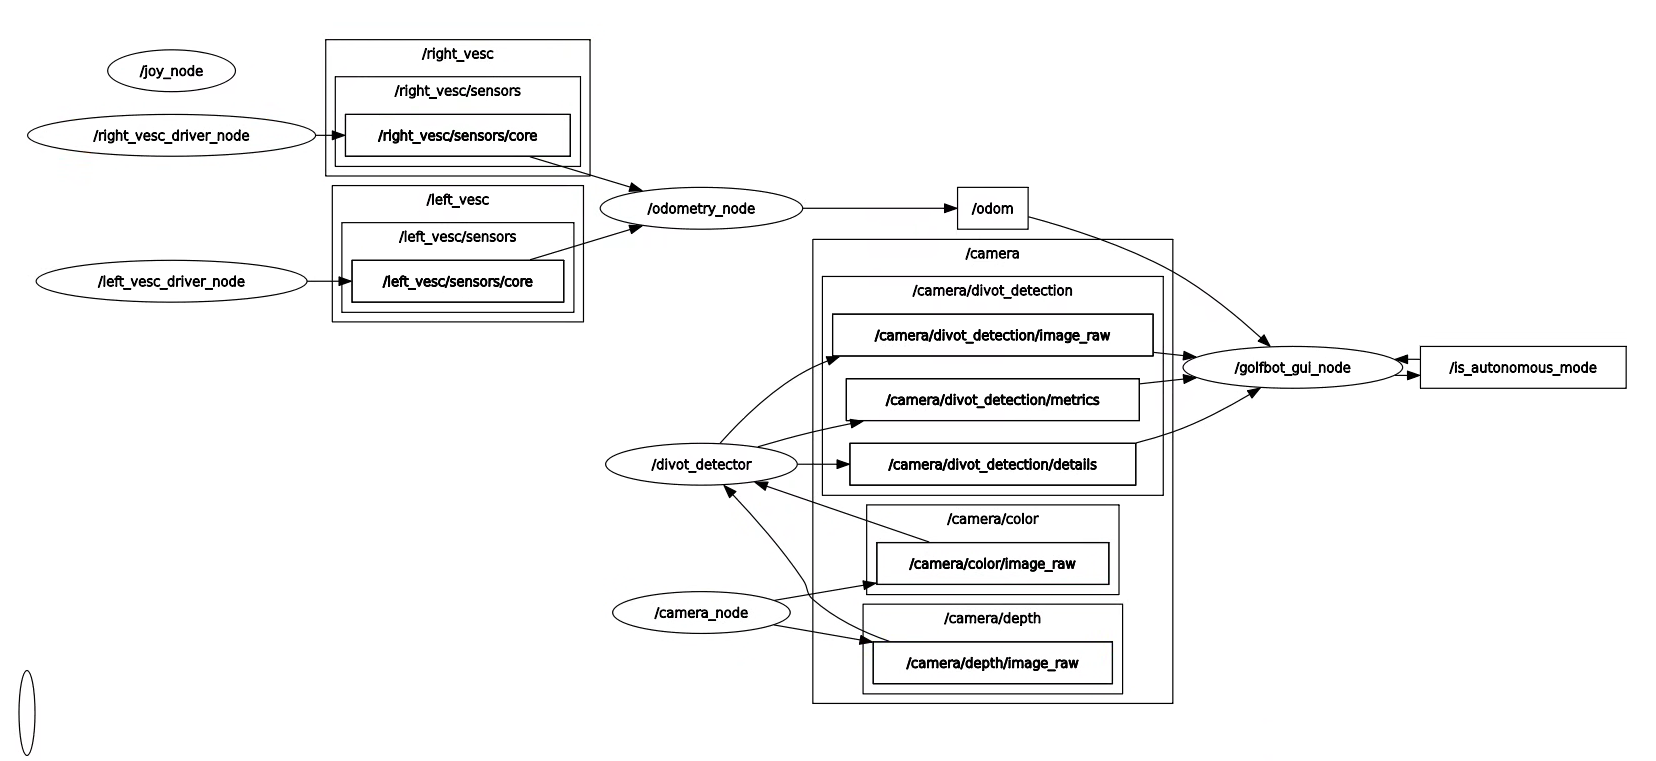
\includegraphics[width=1.0\paperwidth]{figures/ros2_nodes.png}}
    \caption{The ROS 2 computation graph (\texttt{rqt\_graph}) of the running system.}
    \label{fig:appendix_rqt_graph}
\end{figure}

% \begin{figure}[h!]
%     \centering
%     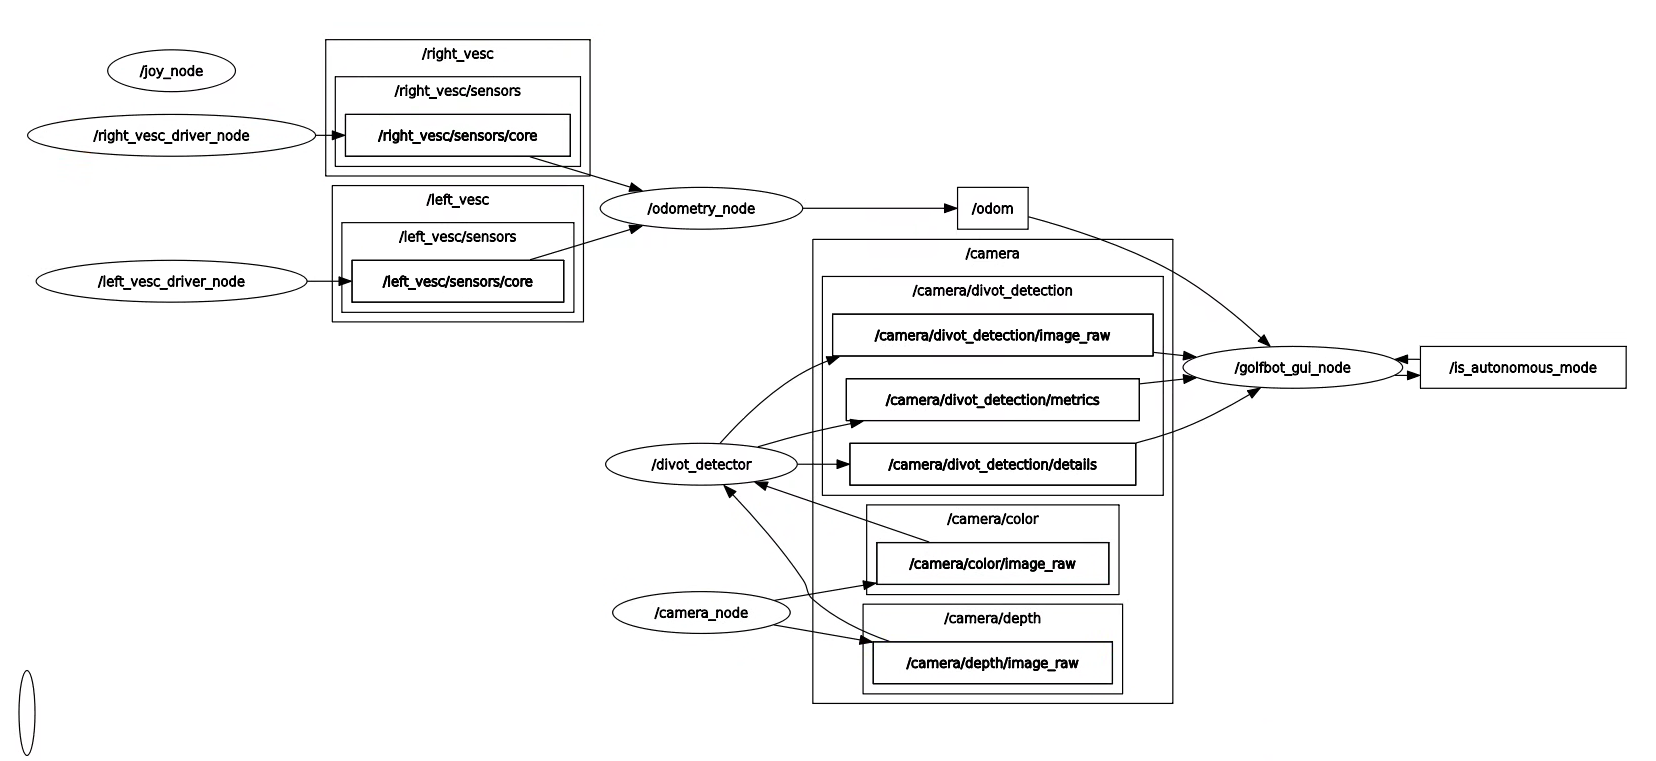
\includegraphics[width=\linewidth]{figures/ros2_nodes.png}
%     \caption{The ROS 2 computation graph of the running GolfBot system.}
%     \label{fig:appendix_rqt_graph}
% \end{figure}

\cleardoublepage % Start the next section on a fresh page

% SECTION 2: Referenced from Section 4.1
\section{Initial Platform Modifications}
\label{sec:appendix_platform_mods}
As mentioned in Chapter \ref{chap:implementation}, several modifications were required to prepare the Wumpus platform for this project. The following figures provide visual evidence of these changes.

\begin{figure}[h!]
    \centering
    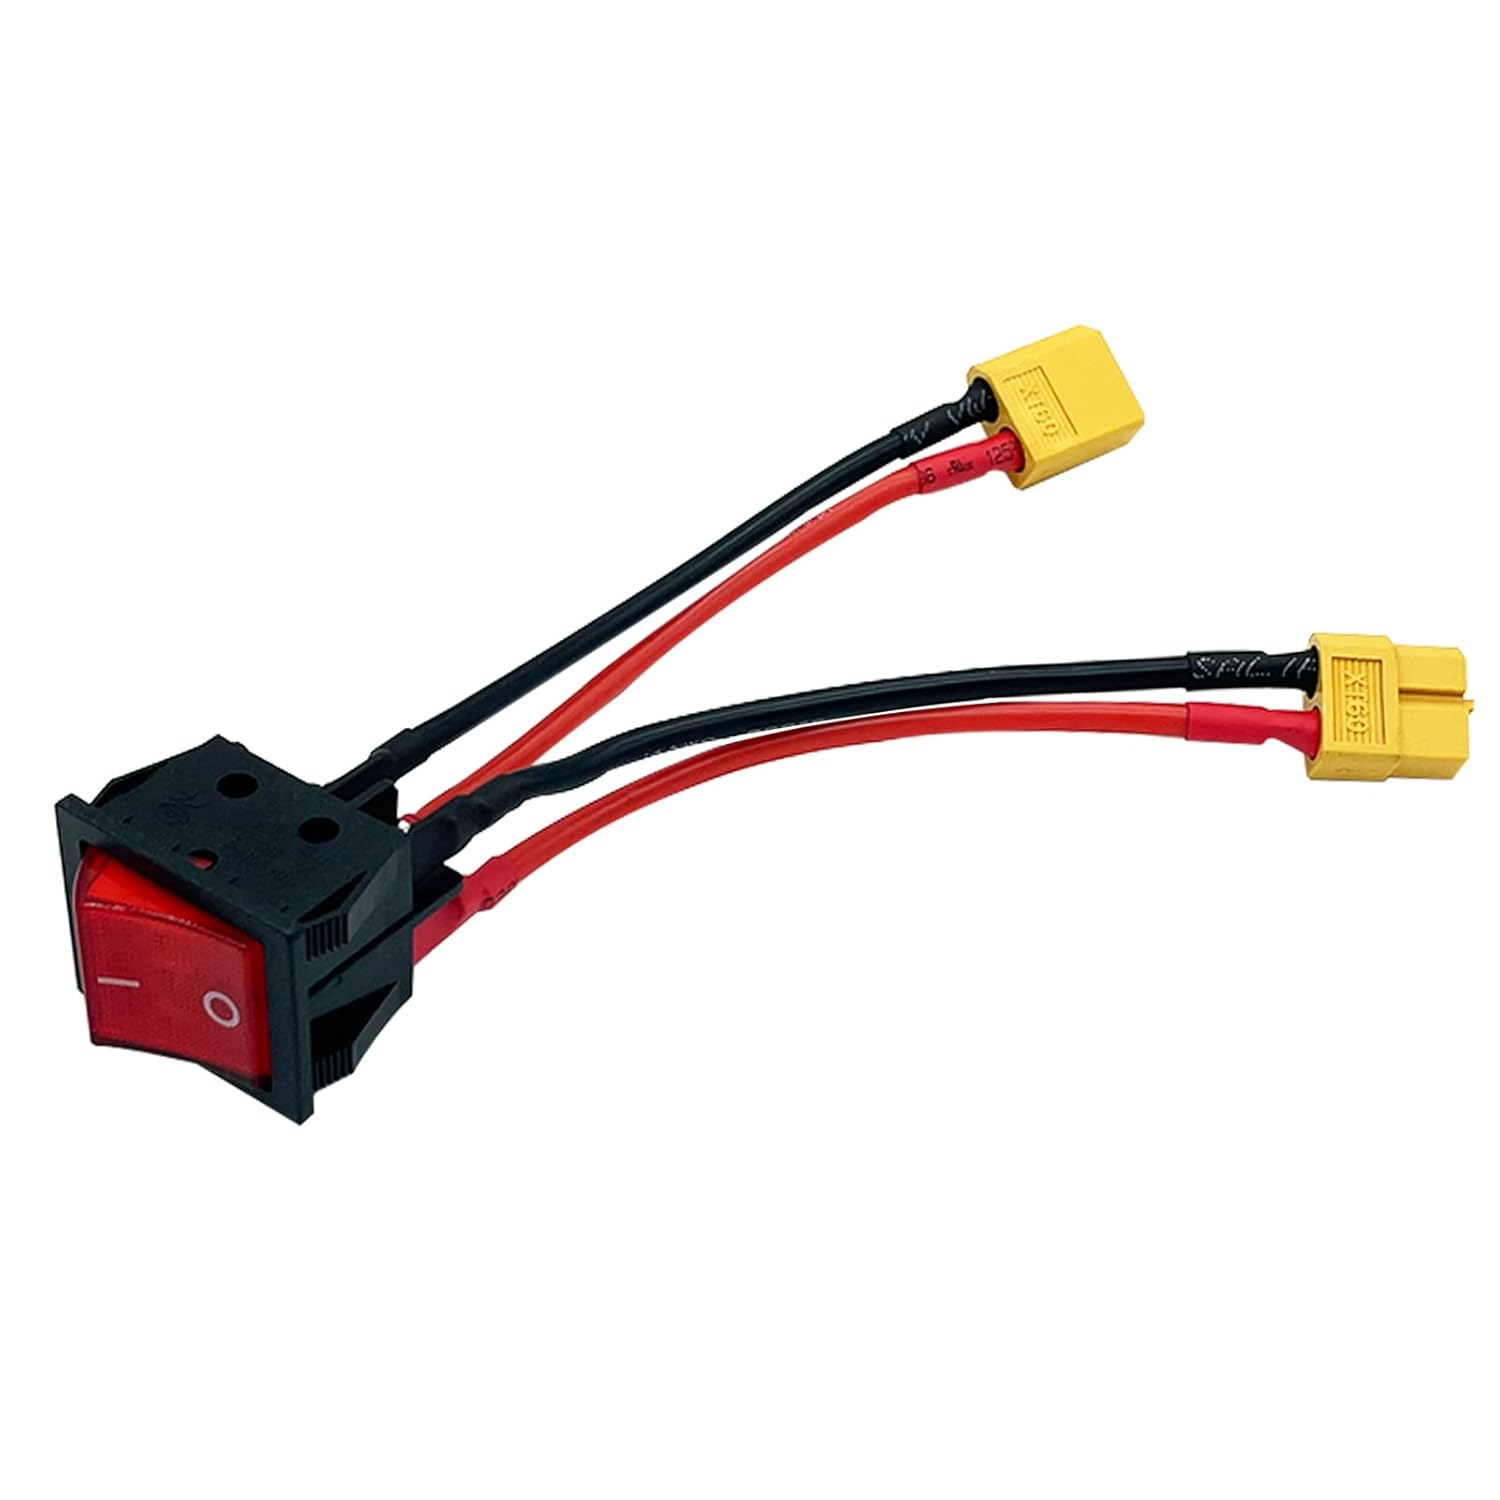
\includegraphics[width=0.4\linewidth]{figures/killswitch.PNG}
    \caption{The dedicated kill switch installed to control the power flow to one of the VESC motor controllers. This modification resolved a recurring power-up issue and improved system safety.}
    \label{fig:appendix_killswitch}
\end{figure}

\begin{figure}[h!]
    \centering
    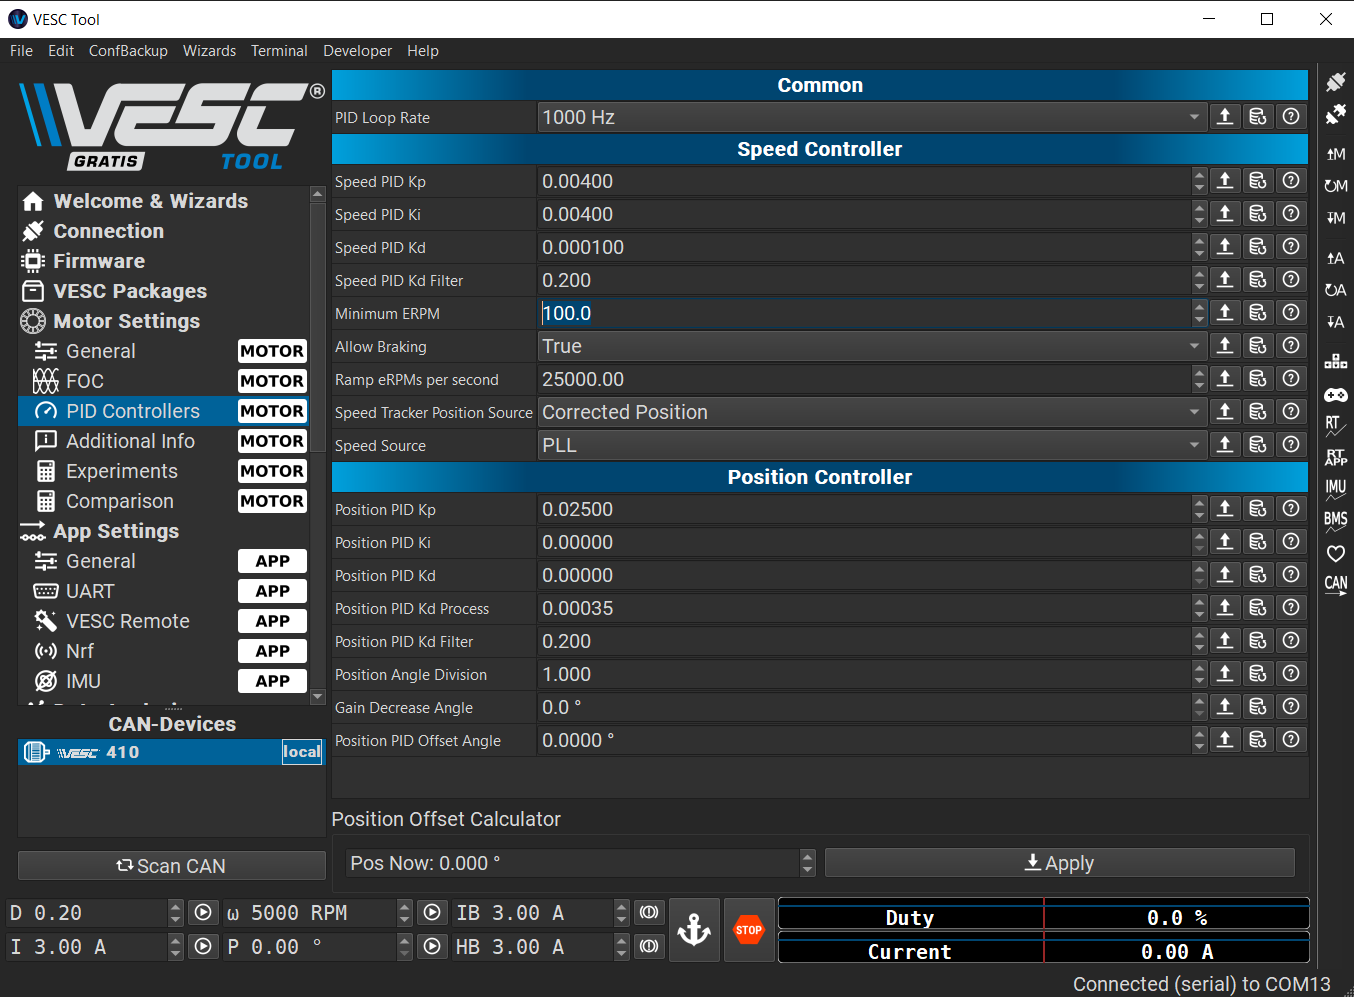
\includegraphics[width=0.8\linewidth]{figures/vesctool.PNG}
    \caption{A screenshot of the VESC Tool software interface. The highlighted field shows the minimum motor speed ("Min ERPM") being adjusted to 100.}
    \label{fig:appendix_vesc_tool}
\end{figure}

\cleardoublepage % this is to start the next section on a new page 

% SECTION 3: Referenced from Section 4.2.2
\section{Data Collection Sample Images}
\label{sec:appendix_dataset_samples}
The following figures show examples of the high-resolution images captured for the two main classes in the custom dataset: \texttt{divot} and \texttt{fixed\_divot}. These raw images formed the basis for the annotation and training process described in Section \ref{ssec:cv_dataset}.

\begin{figure}[h!]
    \centering
    \includegraphics[width=0.8\linewidth]{figures/divot.PNG}
    \caption{An example image from the custom dataset showing the \texttt{divot} class. Note the exposed soil, displaced turf, and distinct textural difference from the surrounding grass.}
    \label{fig:appendix_divot_sample}
\end{figure}

\begin{figure}[h!]
    \centering
    \includegraphics[width=0.8\linewidth]{figures/fixed_divots.PNG}
    \caption{An example image from the custom dataset showing the \texttt{fixed\_divot} class. The area has been filled with a sand-seed mixture, presenting a different color and texture profile for the model to learn.}
    \label{fig:appendix_fixed_divot_sample}
\end{figure}

\cleardoublepage % Start this on a new page

\section{Key Code Snippets}
\label{sec:appendix_code}
This section provides key code snippets from the core ROS 2 nodes to illustrate their implementation logic.

% SECTION 4: Referenced from Section 4.2.5
\subsection{Camera Node - Frame Processing}
Listing \ref{lst:camera_node} shows the main processing loop from the \texttt{camera\_node}. This function is responsible for waiting for new frames from the RealSense camera, aligning the depth and color streams, and publishing the resulting images as ROS 2 topics.

% Note: The 'caption' goes below a listing.
\begin{lstlisting}[language=Python, caption={Core frame processing logic from \texttt{camera\_node.py}.}, label={lst:camera_node}]
def process_frames(self):
    """Processes and publishes camera frames."""
    try:
        frames = self.pipeline.wait_for_frames(timeout_ms=1000)
        if not frames:
            return
        
        # Align frames
        aligned_frames = self.align.process(frames)
        depth_frame = aligned_frames.get_depth_frame()
        color_frame = aligned_frames.get_color_frame()
        
        if not depth_frame or not color_frame:
            return
            
        # Convert to numpy arrays
        color_image = np.asanyarray(color_frame.get_data())
        depth_image = np.asanyarray(depth_frame.get_data())
        
        # Publish raw images
        self.publish_images(color_image, depth_image)
        
    except Exception as e:
        self.get_logger().error(f"Error processing frames: {e}")
\end{lstlisting}

\subsection{Divot Detector Node - Image Callback}
Listing \ref{lst:detector_node} presents the image callback function from the \texttt{divot\_detector\_node}, which contains the primary logic of the computer vision pipeline. This function is triggered whenever a new image is received. It runs the YOLO model, processes the detections using the \texttt{supervision} library, calculates location and size metrics, and publishes the annotated results.

\begin{lstlisting}[language=Python, caption={Primary image callback and processing logic from \texttt{divot\_detector\_intel.py}.}, label={lst:detector_node}]
def image_callback(self, msg: Image):
    try:
        # Convert ROS Image message to OpenCV image
        cv_image = self.bridge.imgmsg_to_cv2(msg, "bgr8")
    except Exception as e:
        self.get_logger().error(f"Could not convert image: {e}")
        return

    # Perform inference silently
    results = self.model(cv_image, verbose=False)[0]
    detections = sv.Detections.from_ultralytics(results)

    # --- Publish Detection Details ---
    # (Code for processing and publishing details...)

    # Annotate the frame with detections
    annotated_frame = self.mask_annotator.annotate(
        scene=cv_image.copy(),
        detections=detections
    )
    # (Further annotation code...)

    # --- NEW: Calculate and display real-world distance ---
    if self.latest_depth_image is not None:
        # (Code for area, volume, and offset calculations...)
        
    try:
        # Convert annotated frame back to ROS Image message and publish
        annotated_msg = self.bridge.cv2_to_imgmsg(annotated_frame, "bgr8")
        annotated_msg.header = msg.header
        self.annotated_image_publisher.publish(annotated_msg)
    except Exception as e:
        self.get_logger().error(f"Could not publish annotated image: {e}")
\end{lstlisting}
